\documentclass{CompilerAssignment}
\usepackage{tikz}

\usetikzlibrary{arrows,shapes,chains}
\title{Assignment 1}

\begin{document}
\maketitle
\section{Exercise 1}

When compiling the given statement,
7 tokens will be generated.
The 1st token is the keyword \verb|int|,
the 2nd token is the identifier \verb|a3|,
the 3rd token is the operator \verb|=|,
the 4th token is the identifier \verb|a|,
the 5th token is the operator \verb|*|,
the 6th token is the integer literal \verb|3|,
and the 7th token is the delimiter \verb|;|.

\section{Exercise 2}

In a string of length $n$, there are

\begin{enumerate}
    \item $n+1$ prefixes;
    \item $n-1$ proper prefixes;
    \item 1 prefix of length $m$;
    \item 1 suffix of length $m$;
    \item 1 (if $m \neq n$) or 0 (if $m = n$) proper prefix of length $m$;
    \item $\dfrac{n(n+1)}{2}+1$ substrings;
    \item $2^n$ subsequences.
\end{enumerate}

\section{Exercise 3}

\begin{enumerate}
    \item $\left(\left(\varepsilon|a\right)^*b^*\right)^*$ denotes the language of all strings over the alphabet $\{a, b\}$.
    \item $\left(a|b\right)^*a\left(a|b\right)\left(a|b\right)$ denotes the language of all strings over the alphabet $\{a, b\}$ that end with $aaa$, $aab$, $aba$ or $abb$.
    \item $a^*ba^*ba^*ba^*$ denotes the language of all strings over the alphabet $\{a, b\}$ where character $b$ appears exactly 3 times.
\end{enumerate}

\section{Exercise 4}

\begin{enumerate}
    \item $86\text{-}0755\text{-}[1-9][0-9]^7$;
    \item $a\left(a|b\right)^*b$;
    \item Let $consonant \rightarrow \left(b|c|d|f|g|h|j|k|l|m|n|p|q|r|s|t|v|w|x|y|z\right)^*$,
    the regular expression is \\
    $consonant\,\mathbf{a}\,consonant\,\mathbf{e}\,consonant\,\mathbf{i}\,consonant\,\mathbf{o}\,consonant\,\mathbf{u}\,consonant$.
\end{enumerate}

\section{Optional Exercise 1}

The DFA for the language of all strings over $\Sigma$ without repeated letters is shown in \cref{fig:dfa}.

\begin{figure}[h]
    \centering
    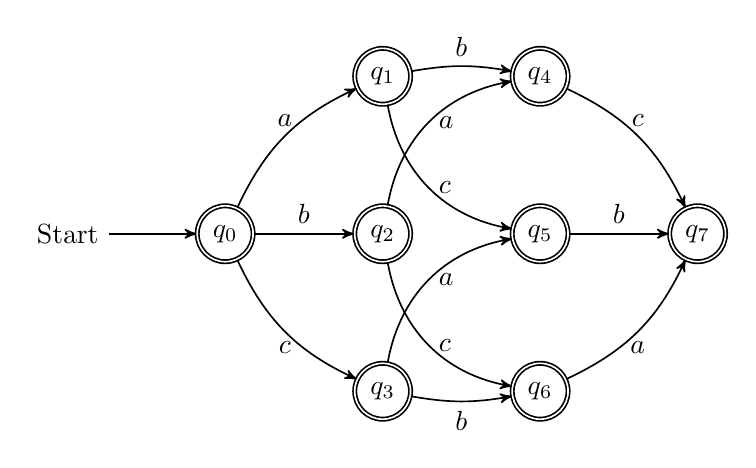
\begin{tikzpicture}[->,>=stealth',auto,semithick]
        \node[style={}](Start)at(-2, 0){Start};
        \node[shape=circle,draw=black,style=double](0)at(0, 0){$q_0$};
        \node[shape=circle,draw=black,style=double](1)at(2, 2){$q_1$};
        \node[shape=circle,draw=black,style=double](2)at(2, 0){$q_2$};
        \node[shape=circle,draw=black,style=double](3)at(2, -2){$q_3$};
        \node[shape=circle,draw=black,style=double](4)at(4, 0){$q_5$};
        \node[shape=circle,draw=black,style=double](5)at(4, 2){$q_4$};
        \node[shape=circle,draw=black,style=double](6)at(4, -2){$q_6$};
        \node[shape=circle,draw=black,style=double](7)at(6, 0){$q_7$};
        \path[](Start) edge (0)
        (0) edge [bend left=20] node [above] {$a$} (1)
        (0) edge node [above] {$b$} (2)
        (0) edge [bend right=20] node [below] {$c$} (3)
        (1) edge [bend left=10] node [above] {$b$} (5)
        (1) edge [bend right=35] node [right] {$c$} (4)
        (2) edge [bend left=35] node [right] {$a$} (5)
        (2) edge [bend right=35] node [right] {$c$} (6)
        (3) edge [bend left=35] node [right] {$a$} (4)
        (3) edge [bend right=10] node [below] {$b$} (6)
        (5) edge [bend left=20] node [above] {$c$} (7)
        (4) edge node [above] {$b$} (7)
        (6) edge [bend right=20] node [below] {$a$} (7);
    \end{tikzpicture}
    \caption{The DFA's transition diagram}
    \label{fig:dfa}
\end{figure}

According to the transition diagram, the regular expression for the language of all strings over $\Sigma$ without repeated letters is
\begin{align*}
    \left(\varepsilon|a\right)\left(\varepsilon|b\right)\left(\varepsilon|c\right)| \\
    \left(\varepsilon|a\right)\left(\varepsilon|c\right)\left(\varepsilon|b\right)| \\
    \left(\varepsilon|b\right)\left(\varepsilon|a\right)\left(\varepsilon|c\right)| \\
    \left(\varepsilon|b\right)\left(\varepsilon|c\right)\left(\varepsilon|a\right)| \\
    \left(\varepsilon|c\right)\left(\varepsilon|a\right)\left(\varepsilon|b\right)| \\
    \left(\varepsilon|c\right)\left(\varepsilon|b\right)\left(\varepsilon|a\right).
\end{align*}

\end{document}